\documentclass[a4paper,12pt,twoside,openright]{report}
\usepackage[T1]{fontenc}				% codifica dei font
\usepackage[utf8]{inputenc}				% lettere accentate da tastiera
\usepackage[english, italian]{babel}	% lingue del documento
\usepackage{url}						% per scrivere gli indirizzi internet
\usepackage[italian]{varioref}			% riferimenti completi
\usepackage{indentfirst}				% rientro prima riga del capoverso
\usepackage{microtype}					% migliora riempimento righe
\usepackage{pdfpages}					% per includere frontespizio.pdf
\usepackage[justification=centering]{caption}

% Margini e interlinea
\usepackage[top=1in, bottom=1in, inner=1.2in, outer=1in]{geometry}
\usepackage{setspace} % comandi per interlinea
\onehalfspacing

% Colori
\usepackage{xcolor}

% Codice
\usepackage{listings}
\usepackage{inconsolata} 	% Font Consolas per il codice (monospace)

\lstdefinelanguage[x64]{Assembler} {
	morekeywords={
		% Istruzioni
		movq,movl,movw,movb,
		pushq,popq,
		addb,addl,addw,addq,
		leaq,
		call, retq, ret, iretq, iret,
		cmpb,cmpl,cmpw,cmpq,
		% Registri
		al,ah,ax,eax,rax,
		bl,bh,bx,ebx,rbx,
		cl,ch,cx,ecx,rcx,
		dl,dh,dx,edx,rdx,
		dil,di,edi,rdi,
		sil,si,esi,rsi,
		rbp,rsp,
		r8,r8d,r8w,r8b,r9,r9d,r9w,r9b,
		r10,r10d,r10w,r10b,r11,r11d,r11w,r11b,
		r12,r12d,r12w,r12b,r13,r13d,r13w,r13b,
		r14,r14d,r14w,r14b,r15,r15d,r15w,r15b
	},
	morecomment=[l]{\#},
	morecomment=[l]{//},
	sensitive=false,
	showspaces=false
}

% Impostazioni bibliografia
\usepackage[autostyle,italian=guillemets]{csquotes}
\usepackage[backend=biber]{biblatex}
\addbibresource{references.bib}
\setcounter{biburlnumpenalty}{9000}
\setcounter{biburlucpenalty}{9000}
\setcounter{biburllcpenalty}{9000}

% Segnalibri e collegamenti
\usepackage[bookmarks]{hyperref}
\usepackage{bookmark}

\begin{document}

% Il frontespizio viene importato da un file pdf con una singola pagina
% generato con un file .tex separato
\phantomsection
\begin{titlepage}
	\thispagestyle{empty}
	
\includepdf{sezioni-tesi/frontespizio/frontespizio-frn.pdf}
	\thispagestyle{empty}	% non numerare questa pagina
	\cleardoublepage
\end{titlepage}

\tableofcontents

\chapter{Meltdown e il sistema di protezione KAISER}
La sicurezza dei sistemi informatici attuali si fonda sull'isolamento della memoria,
ad esempio marcando come privilegiati gli indirizzi di memoria kernel e bloccando eventuali
accessi da parte di programmi utente \cite{lettieri:protezione}. 
\textbf{Meltdown} è un tipo di attacco informatico che sfrutta un effetto
collaterale dell'esecuzione fuori ordine nei processori moderni per leggere locazioni di memoria scelte in maniera
arbitraria. L'attacco funziona su varie microarchitetture Intel prodotte sin dal 2010, indipendentemente dal sistema
operativo in uso. Meltdown è quindi in grado di accedere arbitrariamente a qualsiasi locazione di memoria protetta
(afferenti al kernel o ad altri processi) senza necessitare alcun permesso o privilegio da parte del
sistema \cite{lipp:meltdown}.

Meltdown rompe quindi tutti i meccanismi di sicurezza che si basano sull'isolamento degli spazi di indirizzamento, andando a colpire milioni di utenti. Il sistema di protezione KAISER, sviluppato originariamente per KASLR \cite{gruss:kaslr}, ha l'importante effetto secondario di impedire l'utilizzo di Meltdown \cite{lipp:meltdown}.


\section{Background}

\subsection{Esecuzione Fuori Ordine}
\label{sec:esecuzione-fuori-ordine}

\subsection{Spazi di indirizzamento}
\label{sec:spazi-di-indirizzamento}
\begin{figure}
	\centering
	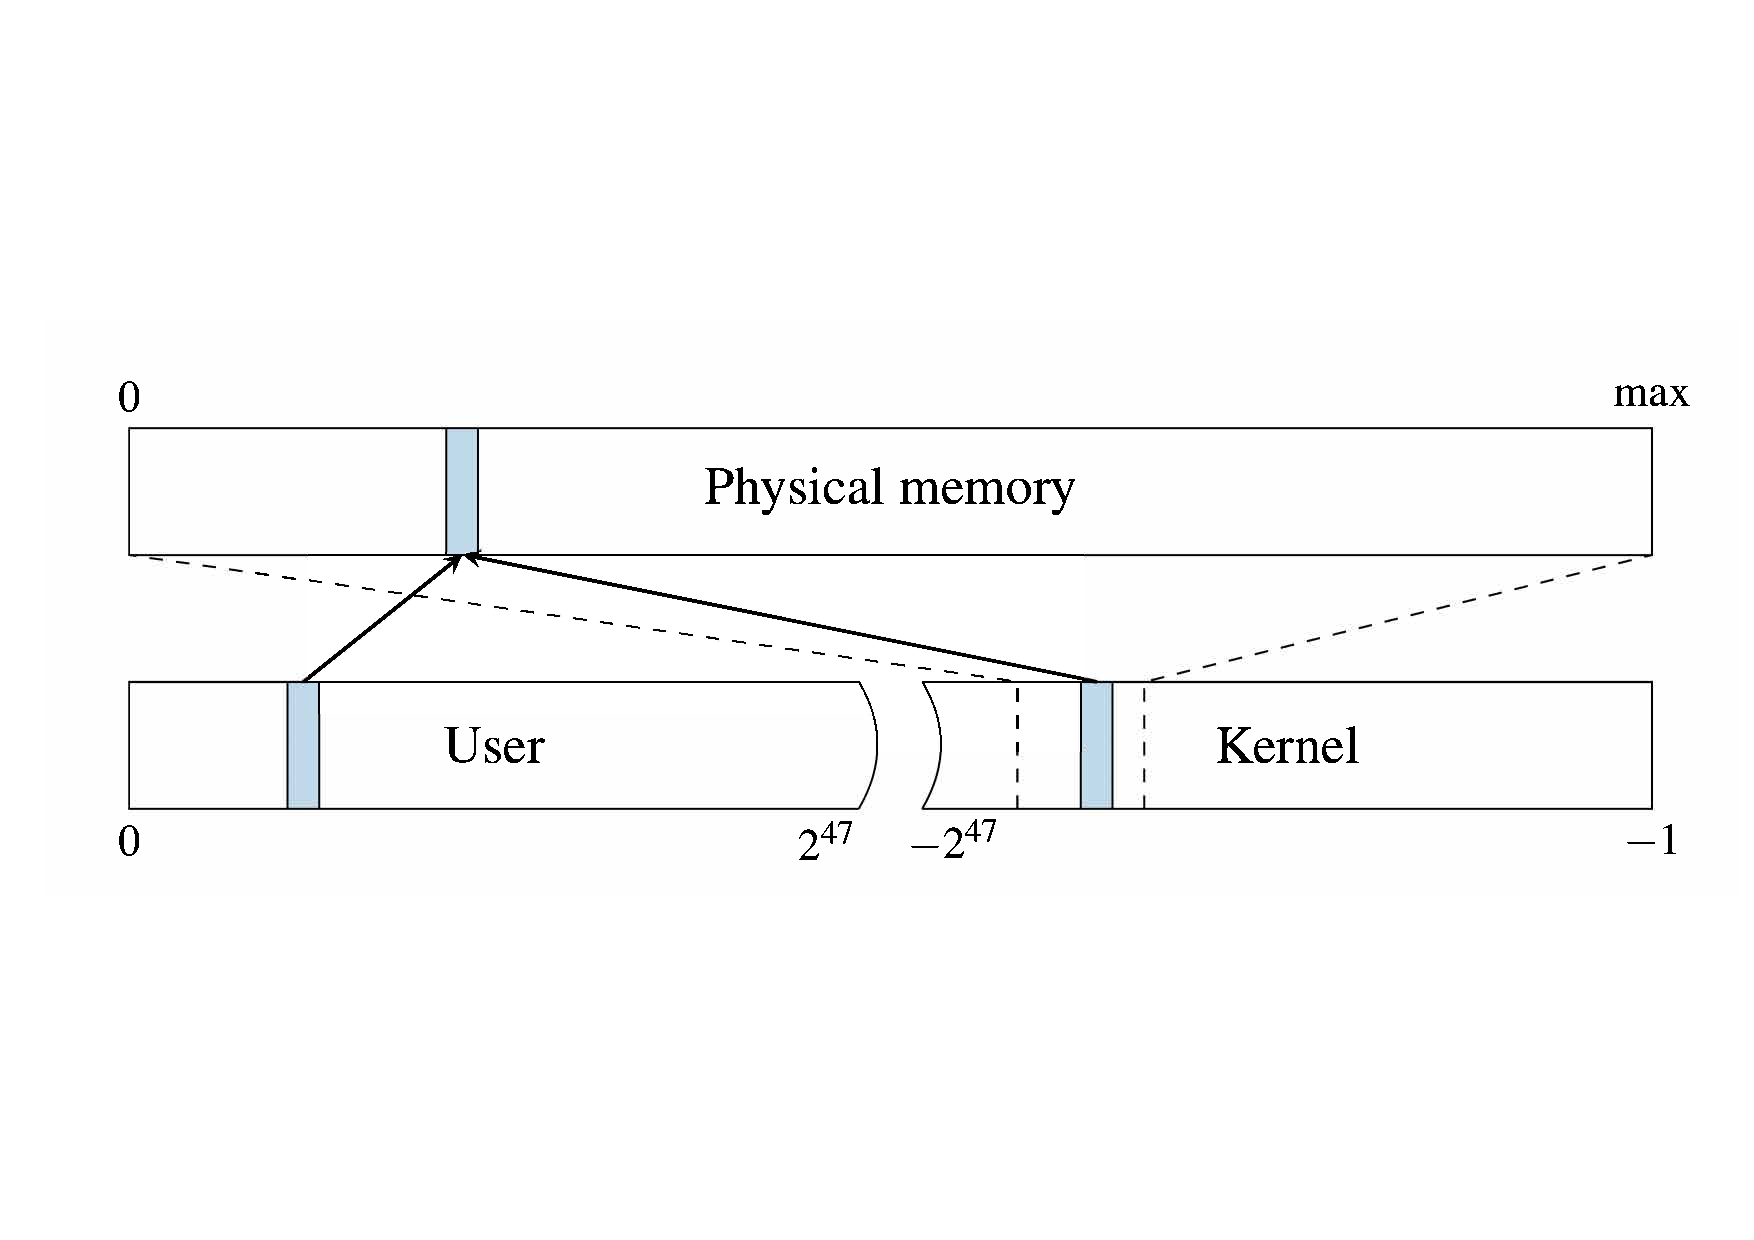
\includegraphics[width=0.5\textwidth]{"img/memoria-fisica.pdf"}
	\caption{text} % TODO
	\label{fig:memoria-fisica}
\end{figure}

Per risolvere diversi problemi, in particolare l'isolamento dei processi \cite{lettieri:paginazione}, le CPU supportano l'utilizzo di spazi d'indirizzamento virtuali, in cui gli indirizzi virtuali (relativi al singolo processo) vengono tradotti in indirizzi fisici. 
Lo spazio d'indirizzamento di un processo (ovvero tutti i possibili indirizzi che un processo può generare) viene suddiviso in regioni dette \emph{pagine} che possono essere mappate individualmente nella memoria fisica attraverso una tabella di traduzione multivello. 
Ogni processo possiede una propria tabella di traduzione che traduce tutti e soli i suoi indirizzi virtuali e che definisce le proprietà di protezione delle varie zone di memoria. 

Ogni processo può quindi riferirsi esclusivamente agli indirizzi appartenenti al proprio spazio di indirizzamento virtuale. Per permettere l'utilizzo 


\subsection{Attacchi Cache}
Al fine di velocizzare gli accessi alla RAM, le CPU contengono buffer di memoria molto veloce ma di dimensioni limitate che costituiscono la cosiddetta \emph{memoria cache}. La memoria cache maschera i tempi di latenza estremamente lunghi per l'accesso alla memoria centrale (molto lenta in confronto alla cache) conservando le locazioni di memoria che, secondo principi statistici come la \emph{località spaziale} (se un programma accede ad un certo indirizzo, è molto probabile che in breve tempo accederà ad un indirizzo vicino)  e la \emph{località temporale} (se un programma accede ad un certo indirizzo, è molto probabile che in breve tempo vi accederà di nuovo), è più probabile vengano indirizzate dalla CPU nel breve periodo \cite{lettieri:cache}.

Gli attacchi a canale laterale (\emph{side-channel attacks}) contro la cache sfruttano questa differenza di tempo di accesso introdotta dalla cache stessa. Negli attacchi Flush+Reload \cite{yaron:flush-reload}, usati da Meltdown \cite{lipp:meltdown}, l'attaccante è in grado di determinare se una locazione di memoria è stata precedentemente caricata in cache, misurando il tempo impiegato da un'operazione di lettura.

%%
\section{Come agisce Meltdown}
L'attacco Meltdown consiste in due fasi fondamentali \cite{lipp:meltdown}:
\begin{enumerate}
	\item Far eseguire alla CPU una o più istruzioni in maniera speculativa (le \emph{transient instruction}) che accedono a locazioni di memoria \textbf{protetta} (kernel o altri processi).
	\item Leggere gli effetti dell'esecuzione delle transient instruction a livello di microarchitettura per ottenere il contenuto delle locazioni di memoria accedute.

\end{enumerate}

\subsection{L'esecuzione delle transient instruction}
Nella prima fase di Meltdown, l'attaccante cerca di accedere ad una zona di memoria protetta, ad esempio la memoria kernel.
Il tentativo di accesso ad una pagina non accessibile da livello utente fa in modo che la CPU sollevi un'eccezione di protezione, che generalmente termina il processo. 
Tuttavia, a causa dell'esecuzione fuori ordine, la CPU potrebbe aver già eseguito l'istruzione di accesso in maniera speculativa \emph{prima} delle istruzioni relative all'eccezione di protezione, al fine di minimizzare i tempi di latenza (vedi paragrafo \ref{sec:esecuzione-fuori-ordine}).
Grazie al lancio dell'eccezione, le eventuali istruzioni eseguite in maniera speculativa, relative dunque ad una previsione di salto \emph{errata}, non vengono ritirate dalla CPU e non hanno così alcun effetto sulla macroarchitettura in generale (memoria centrale e registri logici non speculativi del processore) \cite{frosini:calcolatori2}.

Nonostante non si verificano effetti macroarchitetturali, le transient instruction hanno effetti secondari a livello di \textbf{microarchitettura}. 
Durante l'esecuzione speculativa, la locazione di memoria riferita viene memorizzata sia nella cache che in un registro fisico della CPU. 
Sebbene il loro contenuto non venga mai reso disponibile al programma utente grazie al mancato ritiro delle micro-operazioni, la locazione di memoria resta in cache, diventando possibile vittima di un attacco side-channel alla memoria cache \cite{lipp:meltdown}.

Come abbiamo detto nel paragrafo \ref{sec:spazi-di-indirizzamento}, l'intera memoria fisica viene mappata all'interno dello spazio di indirizzamento del kernel attraversa la cosiddetta \emph{finestra di memoria fisica} \cite{lettieri:paginazione-complementi}.
Essendo la finestra di memoria fisica parte della memoria kernel, dunque, l'attacco Meltdown è in grado non solo di leggere la memoria del kernel, ma anche leggere l'intera memoria fisica, compresi gli spazi virtuali degli altri processi.

\subsection{title}
\label{sec:seconda-fase-meltdown}


\chapter{Introduzione al nucleo didattico}
Il nucleo didattico è un \textbf{kernel a 64 bit} perfettamente funzionante, utilizzato per finalità didattiche nel corso di Calcolatori Elettronici di Ingegneria Informatica presso l'Università di Pisa e sviluppato a partire dai concetti presentati in \citetitle{frosini:calcolatori3} di \citeauthor{frosini:calcolatori3}\cite{frosini:calcolatori3}.

Il sistema è organizzato in tre moduli distinti \cite{lettieri:nucleo}:
\begin{itemize}
	\item \textbf{SISTEMA}, eseguito con il processore a livello sistema, che contiene la realizzazione dei processi, inclusa la gestione della memoria;
	\item \textbf{IO}, eseguito con il processore a livello sistema, che contiene le routine di ingresso/uscita che permettono di utilizzare le periferiche collegate al sistema;
	\item \textbf{UTENTE}, eseguito con il processore a livello utente, che contiene il programma che il nucleo dovrà eseguire.
\end{itemize}
I moduli sistema e io forniscono un supporto al modulo utente, sotto forma di \emph{primitive} che questo può invocare.

Il sistema sviluppato, per quanto funzionante, non è autosufficiente e per sviluppare i moduli necessita di un altro sistema di appoggio, nel nostro caso Linux, i cui strumenti devono essere opportunamente configurati in modo che produca eseguibili per il nostro sistema. Il nucleo così sviluppato può essere eseguito sia su una macchina reale (sconsigliato), sia su un emulatore. Nel nostro caso, useremo una versione di QEMU opportunamente modificata~\cite{lettieri:istruzioni-nucleo}.

Il modulo sistema deve essere caricato da un \emph{bootstrap loader} mentre il modulo io e utente devono essere caricati da una \emph{partizione di swap}, nel nostro caso emulata da un file binario

\section{Gestione dei processi}
All'interno del nucleo didattico, i processi vengono rappresentati attraverso due strutture dati:
\begin{itemize}
	\item Il descrittore di processo (\emph{des\_proc}), contenente il TSS del processo e i valori dei registri salvati all'ultimo cambio di contesto. Viene indirizzato dalla entrata della GDT relativa al processo.
	\item Il \emph{proc\_elem}, contenente l'id e la priorità del processo e usato nelle code di processi.
\end{itemize}

Il sistema prevede una politica di schedulazione a priorità fissa, in cui passa in esecuzione il processo pronto con priorità \emph{maggiore}. A parità di priorità, viene adottata una politica FIFO (\emph{First Input, First Output}).

\section{Gestione della memoria virtuale}
Il nostro sistema implementa la paginazione su domanda~\cite{lettieri:paginazione-su-domanda}, con zone di memoria condivise tra tutti i processi e zone private ai processi~\cite{lettieri:paginazione-nel-nucleo}.

\begin{figure}
	\centering
	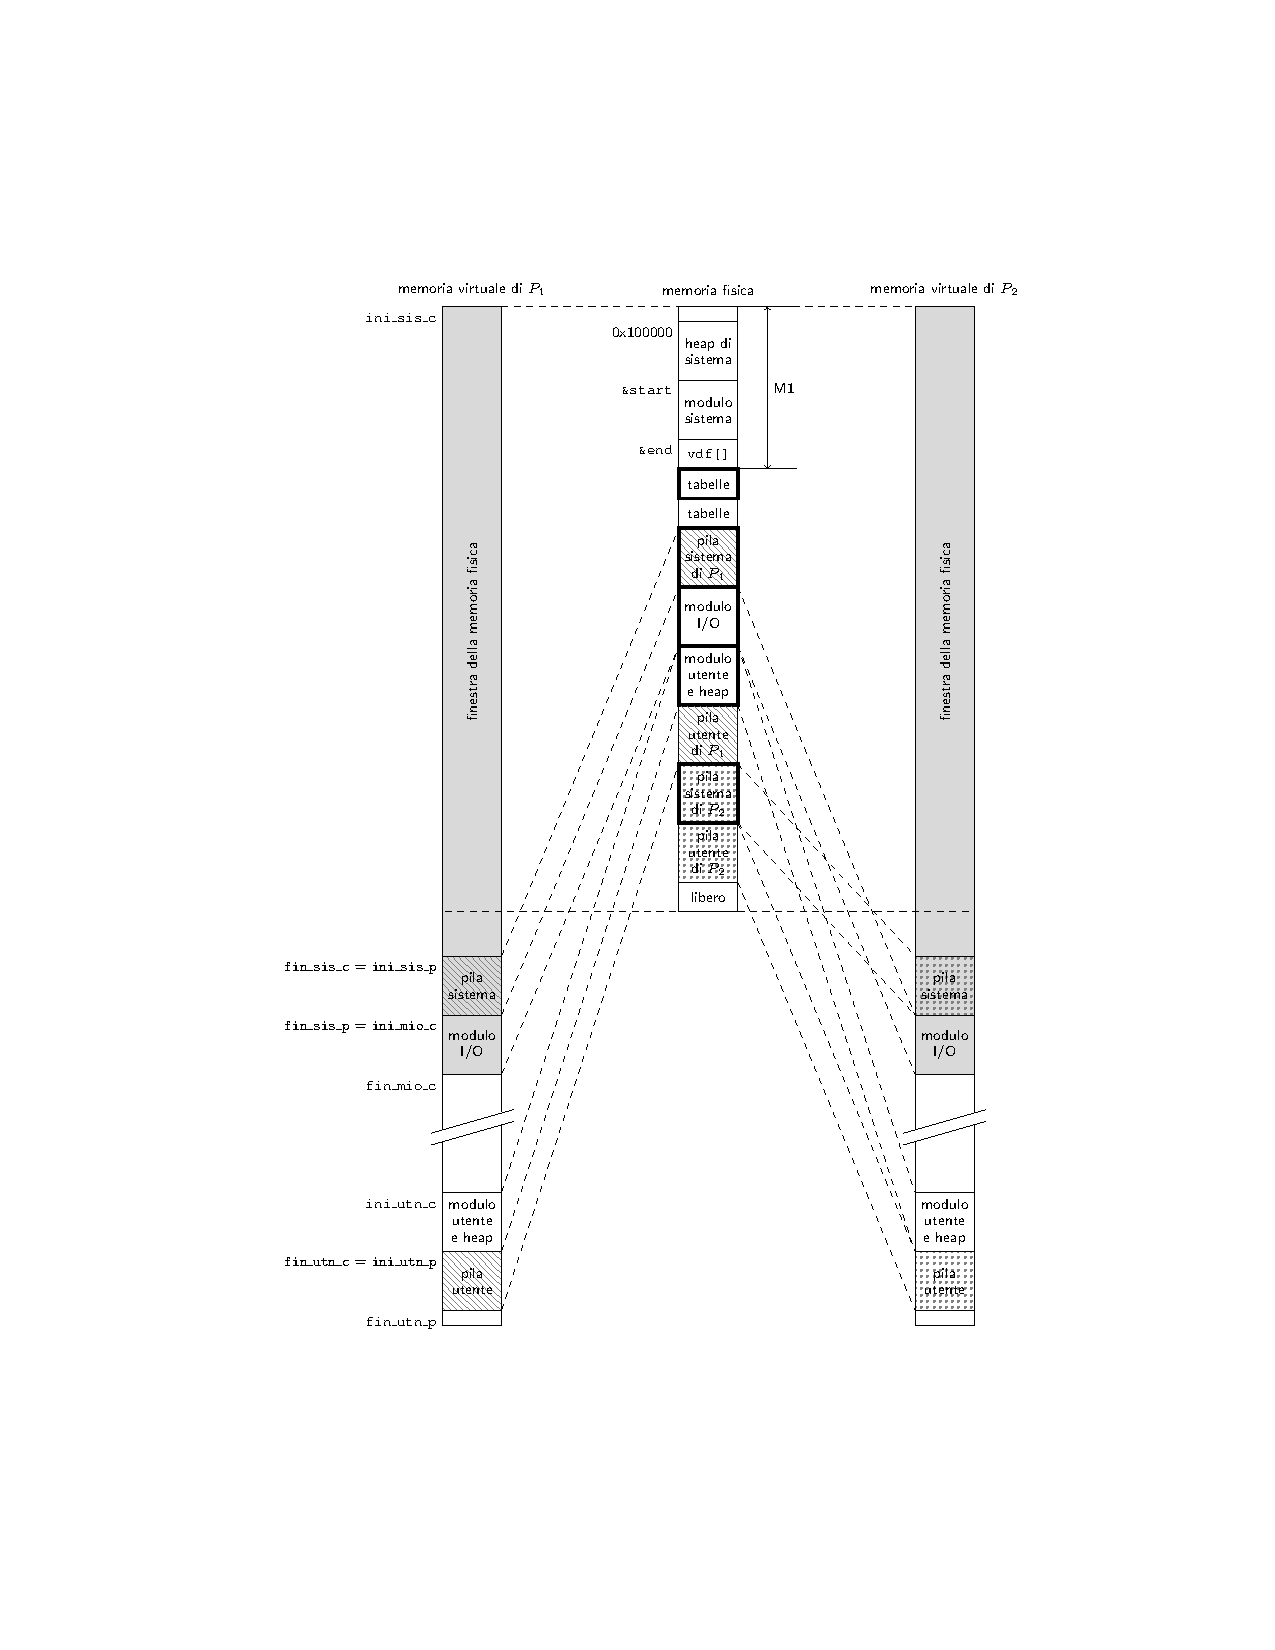
\includegraphics[width=\textwidth]{"img/memoria-virtuale-nucleo.pdf"}
	\caption{Esempio di memoria virtuale con due processi (non in scala)~\cite{lettieri:paginazione-nel-nucleo}}
	\label{fig:memoria-virtuale-nucleo}
\end{figure}

La memoria virtuale di ogni processo è diviso nelle seguenti sezioni (vedi anche \ref{fig:memoria-virtuale-nucleo}: 
\begin{itemize}
	\item Il sottospazio canonico superiore, con indirizzi da 0X0000000000000000 a 0X00007FFFFFFFFFFF, accessibile solo da livello sistema. A sua volta suddiviso in:
	\begin{itemize}
		\item \textbf{sistema/condivisa}: contiene la finestra di memoria fisica
		\item \textbf{sistema/privata}: contiene la pila sistema del processo
		\item \textbf{IO/condivisa}: contiene il modulo I/O
	\end{itemize}
	\item Il sottospazio canonico inferiore, con indirizzi da 0XFFFF800000000000 a 0XFFFFFFFFFFFFFFFF, accessibile solo da livello sistema. A sua volta suddiviso in:
	\begin{itemize}
		\item \textbf{utente/condivisa}: contiene il modulo utente, ovvero le sezioni \texttt{.text} e \texttt{.data} del programma utente
		\item \textbf{utente/privata}: contiene la pila utente del processo
	\end{itemize}
\end{itemize}
Si noti come alcune parti della memoria fisica siano accessibili esclusivamente tramite la finestra: il primo MiB riservato per ragioni storiche, lo heap di sistema, il modulo sistema, i descrittori di frame e i descrittori di pagine virtuali.

Usando la paginazione su domanda, la memoria fisica funziona da cache dello swap. Normalmente le sole sezioni \emph{residenti}, ovvero non selezionabili come vittime per uno swap, sarebbero la \emph{sistema/condivisa} e la \emph{sistema/privata}, in quanto contenenti la finestra di memoria e la pila usata dal modulo sistema. Per semplicità di implementazione, nel nostro sistema sono state rese residenti tutte le sezioni condivise~\cite{lettieri:paginazione-nel-nucleo}.


\chapter{Implementazione del sistema di protezione}
Nello svolgimento di questa tesi, abbiamo implementato sul nostro sistema una versione modificata di KAISER per proteggere il nucleo da Meltdown. 
Per semplicità, è stato protetta soltanto la sezione \emph{sistema/condivisa} della memoria virtuale, contenente la finestra di memoria virtuale (vedi sezione \vref{sec:nucleo-memoria}).
Le sezioni io/condivisa e sistema/privata sono dunque ancora vulnerabili a Meltdown.

\section{La finestra di memoria fisica}
Nel nostro sistema, la finestra di memoria virtuale occupa interamente la \emph{prima} entrata della tabella di livello 4 di ogni processo ed è inizializzata dal boot loader all'avvio della macchina virtuale.
Grazie a questa proprietà, abbiamo potuto effettuare una prima ottimizzazione rispetto alla versione di KAISER proposta da \textcite{gruss:kaslr}: invece di creare lo spazio d'indirizzamento shadow a partire dalla tabella di livello 4, nel nostro sistema viene costruita a partire dalla \emph{tabella di livello 3}.
Al momento del passaggio nelle funzioni trampolino, il sistema modificherà la prima entrata della tabella di livello 4 del processo in esecuzione invece del registro CR4, inserendovi l'indirizzo della tabella di livello 3 "kernel" (se il processore sta passando a livello sistema) o "shadow" (se sta tornando a livello utente).

Oltre al risparmio di spazio per avere una tabella duplicata in meno, questa ottimizzazione evita lo svuotamento implicito del \emph{Translation Lookaside Buffer} (TLB) dovuto alla modifica del registro CR4~\cite{gruss:kaslr}, che avrebbe un impatto negativo sulle prestazioni. 
Nella proposta di \textcite{gruss:kaslr}, questo problema veniva aggirato sfruttando alcune funzionalità delle CPU moderne di cui non disponiamo nel nostro sistema emulato.

\section{Le funzioni e la memoria trampolino}
Nel paragrafo \vref{sec:kaiser} abbiamo affermato che alcune porzioni del kernel devono essere mappate nello spazio di indirizzamento shadow per permettere il funzionamento delle interruzioni.
Nella nostra implementazione le porzioni necessarie (che abbiamo denominato nel loro complesso come \emph{memoria trampolino})sono state raccolte in tre sezioni Assembly: una contenente il codice (\texttt{.trampoline\_text}) e due contenenti i dati (\texttt{.trampoline\_data} per le variabili non costanti e \texttt{.trampoline\_bss} per le costanti).
Ogni sezione è stato allineata alla dimensione delle pagine virtuali (4KiB), in modo che le pagine in cui si trovano le tre sezioni siano occupate da esse in maniera esclusiva e non vi si trovino altre porzioni del kernel.
Questo ci permette di inserirne la traduzione da indirizzo virtuale a fisico nello spazio di indirizzamento shadow.

Le funzioni trampolino d'ingresso (nel kernel) e di uscita (dal kernel) si occupano di aggiornare la prima entrata della tabella di livello 4 con il descrittore di tabella 3 opportuno.
Mentre la tabella di livello 3 \emph{kernel} viene creata dal boot loader, la tabella di livello 3 \emph{shadow} viene creata dal nostro programma durante la fase di inizializzazione della memoria virtuale (vedi sezione \vref{sec:memoria-shadow}) e il suo descrittore viene conservato nella variabile globale \texttt{des\_finestra\_shadow} (riga 754 del listato \ref{lst:sistemacpp-743}).
La sostituzione dello spazio di indirizzamento si limita in pratica a scrivere nella prima entrata della tabella di livello 4 del processo in esecuzione il contenuto di \texttt{des\_finestra\_shadow}, se stiamo passando al livello utente, o di \texttt{des\_finestra\_kernel} (inizializzato da noi; riga 1725 del listato \ref{lst:sistemas-685}), se stiamo passando al livello sistema.

\section{Costruzione dello spazio di memoria shadow}
\label{sec:memoria-shadow}

\section{La gestione dei TSS}

\section{Il TLB}
Nonostante si sia evitato lo svuotamento implicito del TLB, è in ogni caso necessario invalidarlo forzatamente quando il sistema passa da sistema a utente. 
L'efficacia di KAISER si basa sulla garanzia che nell'albero di traduzione di ogni processo non vi sia il kernel e la finestra di memoria fisica (o la struttura equivalente per lo specifico sistema operativo) quando il processore lavora a livello utente e che \emph{la CPU non abbia nessun altro modo per ottenere le traduzioni degli indirizzi}.
Quando il processore lavora in modalità privilegiata, può accedere all'albero di traduzione completo di finestra di memoria fisica e la traduzione degli indirizzi a cui accede viene conservata nel TLB.

Se gli indirizzi della finestra di memoria non venissero invalidati quando il processore torna a livello utente, un processo attaccante potrebbe accedere tranquillamente agli indirizzi di sistema acceduti dal processore, in quanto, essendo le loro traduzioni conservate nel TLB, il processore \emph{non} utilizzerà l'albero di traduzione, bypassando così la protezione contro Meltdown.

Dunque, è necessario invalidare il TLB nella funzione trampolino di uscita dal kernel (vedi riga 565 del listato \vref{lst:sistemas-519}).

\chapter{Codice}
\label{cap:codice}

\lstdefinestyle{customcpp}{
	language=C++,
	%
	frame=single,
	numbers=left,
	% Margine
	xleftmargin=1.1cm,
	%
	tabsize=4,
	breaklines=true,
	postbreak=\mbox{\textcolor{black}{$\hookrightarrow$}\space},
	% Stile
	basicstyle=\ttfamily\onehalfspacing\footnotesize,
	keywordstyle=\color{black},
	commentstyle=\sc,
	% Codice
	morekeywords={natq, natl, natw, natb, vaddr, addr, "C", tab\_entry}
}

\lstdefinestyle{customasm}{
	language={[x64]Assembler},
	frame=single,
	numbers=left,
	% Margine
	xleftmargin=0.5in,
	%
	tabsize=4,
	breaklines=true,
	postbreak=\mbox{\textcolor{black}{$\hookrightarrow$}\space},
	% Stile
	basicstyle=\ttfamily\onehalfspacing\small,
	keywordstyle=\color{black},
	commentstyle=\sc
}

\section{sistema.cpp}

\lstinputlisting[
	language=C++,
	style=customcpp,
	firstnumber=19,
	label=lst:sistemacpp-19,
	caption={Descrittori di processo e di TSS}
	]{"code/sistema_19.cpp"}

\lstinputlisting[
	language=C++,  
	style=customcpp,
	firstnumber=743,
	label=lst:sistemacpp-743,
	caption=Creazione della finestra di memoria shadow
	]{"code/sistema_743.cpp"}

\lstinputlisting[
	language=C++,  
	style=customcpp,
	firstnumber=1009,
	label=lst:sistemacpp-1009,
	caption=Creazione di un processo
	]{"code/sistema_1009.cpp"}
	
	
\lstinputlisting[
	language=C++,  
	style=customcpp,
	firstnumber=1191,
	label=lst:sistemacpp-1191,
	caption=Distruzione di un processo
	]{"code/sistema_1191.cpp"}

\lstinputlisting[
	language=C++,  
	style=customcpp,
	firstnumber=1838,
	label={lst:sistemacpp-1838},
	caption=Inizializzazione del sistema
	]{"code/sistema_1838.cpp"}

%%
\section{sistema.s}

\lstinputlisting[
	language={[x64]Assembler},  
	style=customasm,
	firstnumber=38,
	label=lst:sistemas-38,
	caption=Salva e carica stato
	]{"code/sistema_38.s"}

\lstinputlisting[
	language={[x64]Assembler},  
	style=customasm,
	firstnumber=333,
	label=lst:sistemas-333,
	caption=Istruzioni per caricare nella GDT le primitive trampolino
	]{"code/sistema_333.s"}
	
\lstinputlisting[
	language={[x64]Assembler},  
	style=customasm,
	firstnumber=364,
	label=lst:sistemas-364,
	caption=Inizializza GDT e TSS
	]{"code/sistema_364.s"}
	
\lstinputlisting[
	language={[x64]Assembler},  
	style=customasm,
	firstnumber=519,
	label=lst:sistemas-519,
	caption=Funzioni trampolino
	]{"code/sistema_519.s"}
	
\lstinputlisting[
	language={[x64]Assembler},  
	style=customasm,
	firstnumber=685,
	label=lst:sistemas-685,
	caption={Esempio della parte Assembly di una routine di sistema \\con le chiamate alle funzioni trampolino}
	]{"code/sistema_685.s"}

\lstinputlisting[
	language={[x64]Assembler},
	style=customasm,
	firstnumber=1666,
	label=lst:sistemas-1666,
	caption=Sezioni DATA e TSS della memoria shadow/trampolino
	]{"code/sistema_1666.s"}

%%
\section{io.s}

\lstinputlisting[
	language={[x64]Assembler},  
	style=customasm,
	firstnumber=378,
	label=lst:ios-378,
	caption={Esempio della parte Assembly di una primitiva di I/O \\ con le chiamate alle primitive trampolino}
	]{"code/io_378.s"}

%%
\section{costanti.h}

\lstinputlisting[
	language=C++,  
	style=customcpp,
	firstnumber=76,
	label=lst:costantih-76,
	caption=Costanti per gli id delle primitive trampoline
	]{"code/costanti_76.h"}

\cleardoublepage
\addcontentsline{toc}{chapter}{Listings}
\lstlistoflistings

\cleardoublepage
\phantomsection
\addcontentsline{toc}{chapter}{\bibname}
\printbibliography

\end{document}
